\section{Проведение эксперимента}
\subsection{Постановка эксперимента}
Для проверки качества и сравнения алгоритмов было поставлено 3 эксперимента:
\begin{itemize}
   \item Построение рекомендаций Байесовским
   персонализированным ранжированием и калибровка методом Кульбака-Лейблера \cite{bib4}.
   \item Построение рекомендаций Байесовским
   персонализированным ранжированием и калибровка методом Сент-Лагю \cite{bib5}.
   \item Построение рекомендаций с помощью готового фреймворка SurPRISE \cite{sur}.
\end{itemize}
\subsection{Набор данных}
Для проведения эксперимента был выбран датасет MovieLens 25M \cite{voc3}, включающий в себя 25 миллионов оценок к 62,000 фильмов от 162,000 пользователей.
Данные представленны в виде двух csv файлах. Первый rating.csv состоит из
четырех колонок: userId -- id пользователя, moviesId -- id фильма, 
rating -- оценка, поставленная по пятибальной шкале, пользователем для данного фильма,
timestamp -- временная отметка оценки.
   \begin{center}
   \begin{tabular}{ | r  | l | l | l |}
      \hline
      userId & movieId & rating & timestamp  \\ \hline
      1 & 2 & 3.5 & 1112486027 \\
      1 & 29 & 3.5 & 1112486676 \\
      1 & 32 & 3.5 & 1112486819\\
      1 & 47 & 3.5 & 1112486727 \\
      1 & 50 & 3.5 & 1112486580 \\
      1 & 112 & 3.5 & 1112486740 \\
      1 & 151 & 4 & 1112486734 \\
      1 & 223 & 4 & 1112486573 \\
      1 & 253 & 4 & 1112486940 \\
      1 & 260 & 4 & 1112486826 \\
      \hline
      \end{tabular}
   \end{center}
Второй файл movies.csv состоит из трех столбцов: moviesId -- id фильма, 
title -- название фильма, genres -- жанры, к которым относится фильм.
   \begin{center}
      \scalebox{0.9}{
      \begin{tabular}{ | r | l | l |}
         \hline
         movieId & title & genres \\ \hline
         1 & Toy Story (1995) & Adventure|Animation|Children|Comedy|Fantasy \\
         2 & Jumanji (1995) & Adventure|Children|Fantasy \\
         3 & Grumpier Old Men (1995) & Comedy|Romance \\
         4 & Waiting to Exhale (1995) & Comedy|Drama|Romance \\
         5 & Father of the Bride Part II (1995) & Comedy \\
         6 & Heat (1995) & Action|Crime|Thriller \\
         7 & Sabrina (1995) & Comedy|Romance \\
         8 & Tom and Huck (1995) & Adventure|Children \\
         9 & Sudden Death (1995) & Action \\
         10 & GoldenEye (1995) & Action|Adventure|Thriller \\
         \hline
         \end{tabular}
      }
      \end{center}

Во фреймворке SurPRISE \cite{sur} встроены несколько наборов данных, например MovieLens 1M, но для 
более честного сравнения, будем вручную загружать набор MovieLens 25M.
\subsection{Результаты}

В результате эксперимента 1 была произведена калибровка рекомендаций и подбор коэффициента $\lambda$ для калибровки Кульбака-Лейблера (\ref{eq:Calibrated})
и были получены следующие результаты:
\begin{center}
   \scalebox{1}{
   \begin{tabular}{ | r | c | l |}
      \hline
      $\lambda$ & Precision & $C_{KL}$ \\ \hline
      ${\lambda =0}$ (нет калибровки) & 0.43 & 0.93 \\
      ${\lambda =0.2}$ & 0.49 & 0.47 \\
      ${\lambda =0.3}$ & 0.45 & 0.39 \\
      ${\lambda =0.5}$ & 0.33 & 0.31 \\
      ${\lambda =0.7}$ & 0.21 & 0.25 \\
      ${\lambda =0.8}$ & 0.18 & 0.11 \\
      ${\lambda =0.99}$ & 0.14 & 0.019 \\
      \hline
      \end{tabular}
   }
   \end{center}
Заметно, что с увеличением $\lambda$ идет уменьшение дивергенции Кульбака-Лейблера между распределениями, следовательно
полученные рекомендации больше поможи на интересы пользователя. Но также 
с увеличением $\lambda$ идет сначала небольшой рост точности, а после ее снижение.
Для наилучшего результата, я считаю оптимальным взять $\lambda=0.3$.

В эксперименте 2 после применения калибровки адаптированным методом Сент-Лагю \cite{bib5}, получились следующие результаты:
\begin{center}
   \scalebox{1}{
   \begin{tabular}{ | r | l |}
      \hline
      Precision & $C_{KL}$ \\ \hline
         0.12 & 0.3 \\
      \hline
      \end{tabular}
   }
   \end{center}
Точность получилась заметно хуже исходной, а сходство полученного
распределения интересов пользователя с реальным заметно меньше, чем 
при калибровке Кульбака-Лейблера с таким же показателем точности.

Эксперимент 3, при использовании готового фреймворка, показал достаточно хорошие результаты:
\begin{center}
   \scalebox{1}{
   \begin{tabular}{ | r | l |}
      \hline
      Precision & $C_{KL}$ \\ \hline
         0.53 & 0.61 \\
      \hline
      \end{tabular}
   }
   \end{center}
этот метод показывает наилучшую точность, но не впечатляющие значения дивергенции Кульбака-Лейблера.

Для более наглядной демонстрации результатов привожу несколько графиков для сравнения распределений интересов пользователя.
На графике отобразим долю каждого жанра среди интересов для пользователей. 
Синим цветом обонзачены исходные данные, на которых обучались алгоримы,
оранжевым цветом обозначены данные, полученные рекомендательной системой,
а зеленым цветом обонзачены откалиброванные данные, сгенерированные рекомендательной системой.
\begin{figure}[ht]
   \begin{flushleft}
      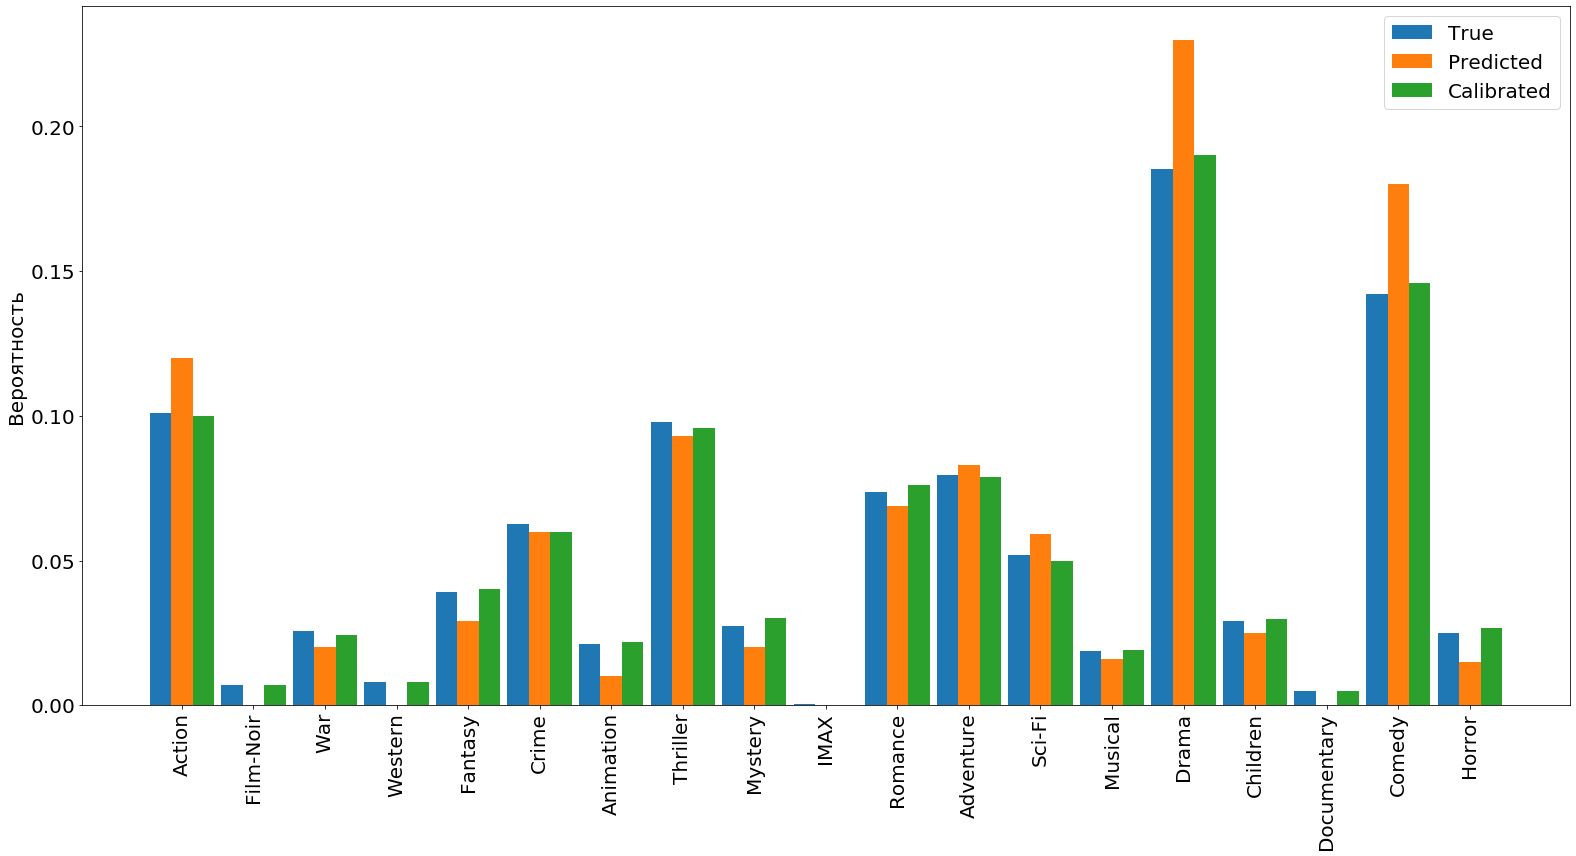
\includegraphics[width=17.5cm, height=10cm]{images/bay.png}
   
   \caption{
   \label{graph-KL}
        Распределение жанров при Байесовском персонализированном ранжировании.}
   \end {flushleft}

   \end {figure}

\pagebreak

На рисунке \ref{graph-KL} демнострируется эффект калибровки Кульбака-Лейблера с ${\lambda=0.3}$ для Байесовского персонализированного ранжирования.
Заметно, что жанры, которые больше остальных представлены в обучающих данных, выдаются рекомендательной системой еще чаще,
в то время как калибровка приближает данные к реальным. С малочисленными жанрами ситуация обстоит немного иначе,
Байесовское персонализированное ранжирование не представило некоторые жанры, например вестерн и документальное кино, калибровка же
исправила это упущение. Таким образом, можно сделать вывод, что калиброванные рекомендации
намного лучше удовлетворяют интересы пользователя.


\pagebreak

   \begin{figure}[ht]
   \begin{flushleft}
      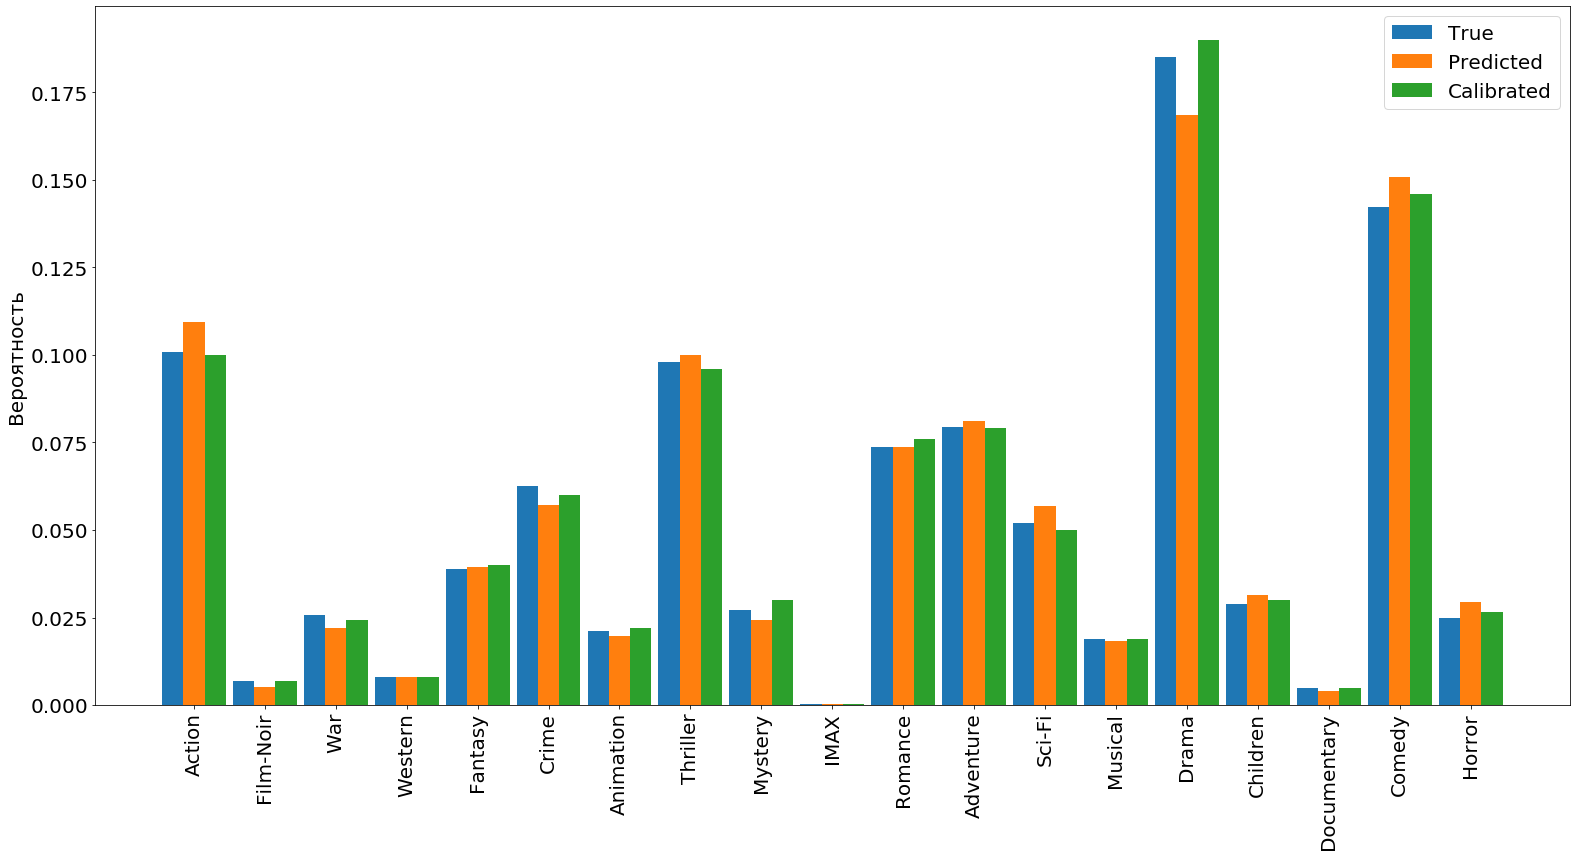
\includegraphics[width=17.5cm, height=10cm]{images/cal_surp.png}
   
   \caption{
   \label{graph-SUR}
        Распределение жанров при использовании фреймворка SurPRISE.}
   \end {flushleft}
   \end {figure}



      На рисунке \ref{graph-SUR} сравниваются распределения, фареймворком SurPRISE и калибровкой Кульбака-Лейблера с ${\lambda=0.3}$ для Байесовского персонализированного ранжирования.
      Тут уже нет серьезных проблем со стороны рекомендательной системы, все жанры представлены и
      имеют долю достаточно близкую к реальной. Калибровка в этом случае показывает все еще лучший результат, но разница уже не так велика.

      По итогам экспериментов, можно сказать, что калибровка показала отличные результаты,
      интересы ползователей удовлетворяются достаточно хорошо и распределение жанров получается близким к реальному.
      Точность при калибровке может немного снизится, но я считаю, что пользовательский опыт при этом не пострадает, так как их интересы будут более широко представлены.


\pagebreak

